\begin{appendices}

\chapter{Dependencies Between City Structure and Thermal Behaviour in Brno}
\label{app:Visualisation}

Results of visualisation are presented in Fig. \ref{fig:Transect1} and Fig. \ref{fig:Transect2}. Both figures have the following structure. A distance along the transect in meters forms a common X axis. A true-colour composition from CASI data is shown in the topmost panel, the transect is drawn with a yellow line. Surface temperatures of a summer day and a summer night are shown in the second panel. Surface temperature of a winter night is shown in the third panel. A depiction of city structure is contained in the fourth panel. Terrain level is shown in brown, while buildings are distinguished from high vegetation with grey and green colours, respectively. NDVI is shown in fifth panel and absorbed energy is shown in the last panel.

Several common observations can be made in both figures. NDVI as a measure of “greenness” follows a classification of high vegetation and also allows distinguishing between streets and a surface covered by grass. Local minima in absorbed energy follow shaded regions at the edges of buildings. Temperature over areas covered by vegetation tends to be more stable and lower in average, while the temperature of streets and parking lots is significantly higher during summer day.

We would like to point out several interesting features in individual transects. We will use an X axis to label the details.

In Figure 1 between 80 and 90, the stabilising role of vegetation can be seen – the temperature profile has a low variability as well as a lower average despite a higher amount of absorbed energy. In Figure 1 at 305 and 390, two different roof surfaces can be observed – the rightmost one is dark, has a high absorptivity, while the leftmost one has a high reflectivity and reflects a cold sky in both summer and winter night. The region from 400 to 550 contains green areas which surrounds Špilberk castle. Summer day temperature is significantly lower in this region compared to other built up areas. The only notable temperature extreme is visible between 460 and 470 where the transect crosses a path walk.

Figure 2 shows interesting features as well. Roofs with high reflectivity can be observed at 160 – 170 and 530 – 540. The coldest places during a summer day are the river between 260 and 280 (which is on the other hand the warmest place in winter) and hard shadows next to high buildings, e.g. at 545. There is a notable shaded hillside between 40 and 50 causing temperature decrease in both summer day and night. There is an interesting dip in the summer night temperature profile between 360 and 370, which is presumably caused by a parked car in the parking lot. A dip in the summer temperature around 445 is caused by a roof window included in the transect.


\newpage
\begin{figure*}[!t]
\centering
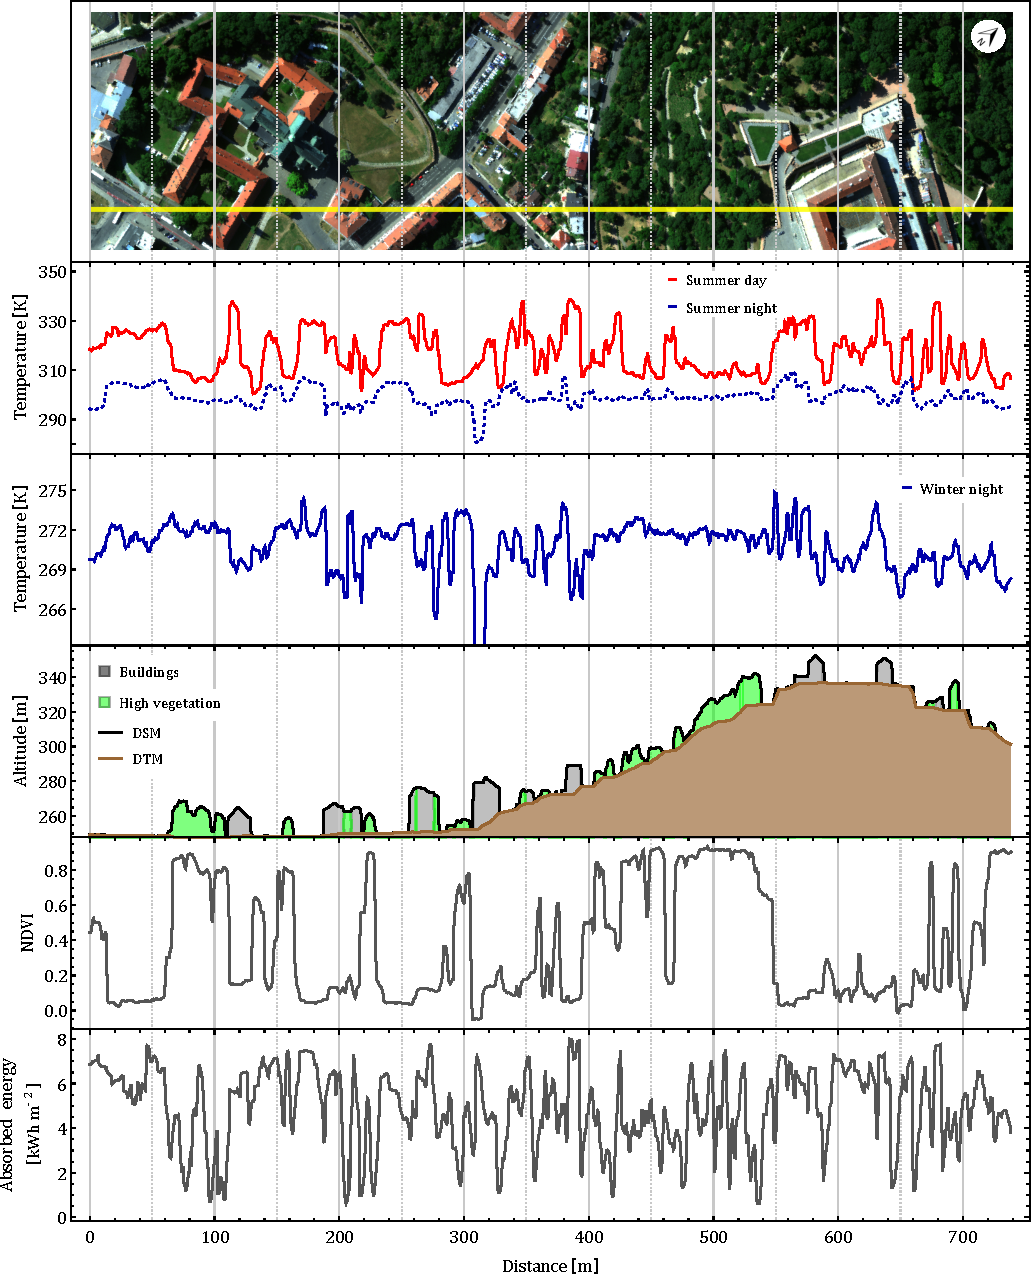
\includegraphics[width=\linewidth]{pics/Appendix_B/Transect_1.pdf}
\vspace{1.5 em}
\caption{TODO.}
\label{fig:Transect1}
\end{figure*}

\newpage
\begin{figure*}[!t]
\centering
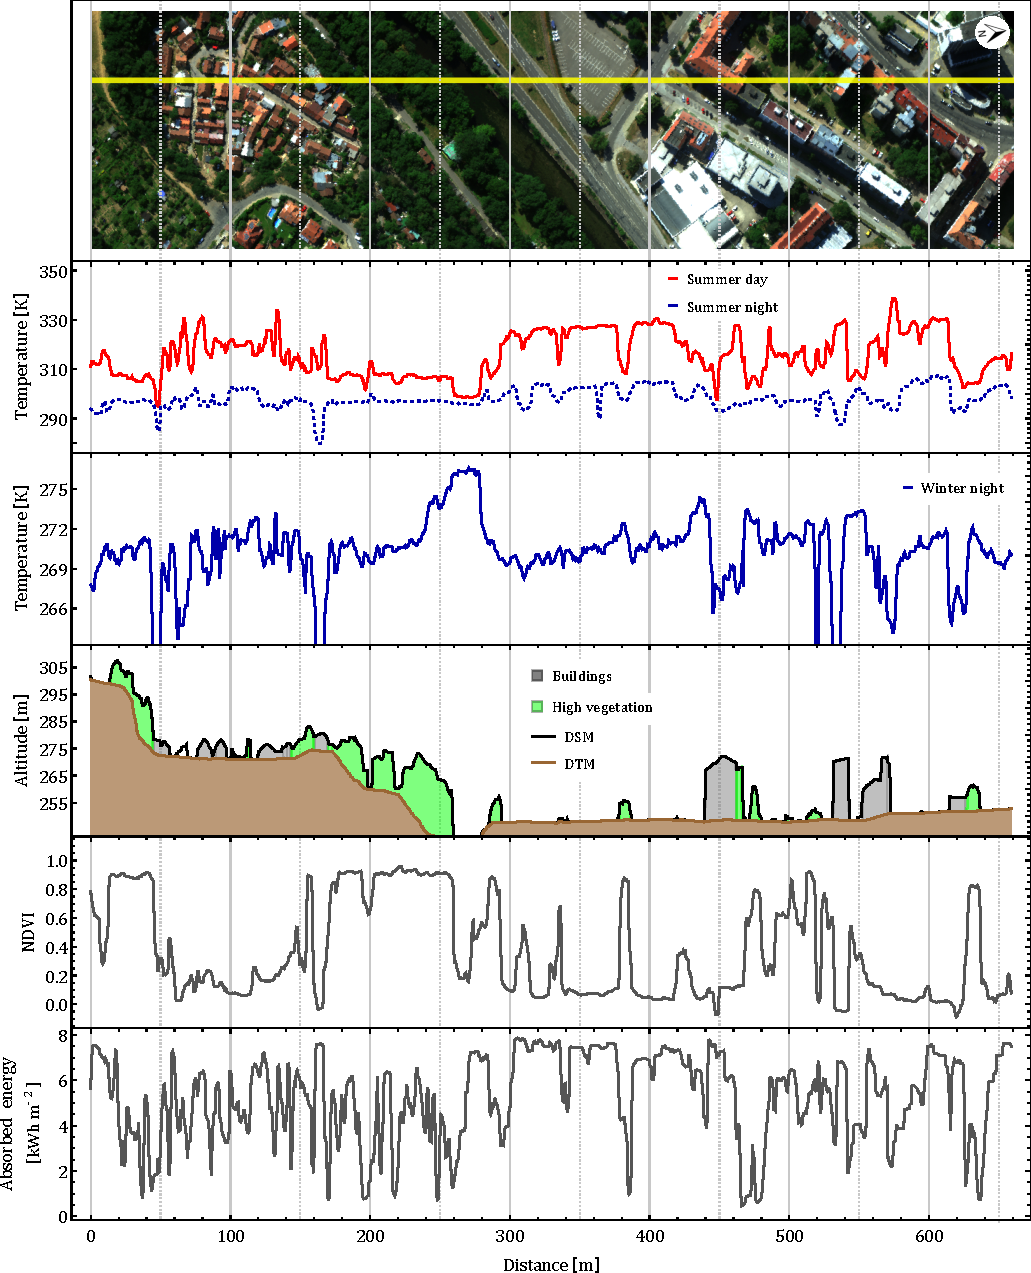
\includegraphics[width=\linewidth]{pics/Appendix_B/Transect_2.pdf}
\vspace{1.5 em}
\caption{TODO.}
\label{fig:Transect2}
\end{figure*}